\documentclass[a4paper,12pt]{book}
\usepackage[spanish,es-tabla]{babel}
\usepackage{blindtext}
\usepackage{graphicx}
\usepackage{subcaption}
\usepackage{caption}
\captionsetup{font={small,it}, labelfont=bf, justification=justified}
\usepackage{amsmath}
\usepackage{tikz}
\usetikzlibrary{arrows.meta,calc,decorations.pathmorphing,shadings}
\usepackage{float}
\usepackage{mathrsfs}%para el tipo de letra \mathscr


\usepackage{color}   %May be necessary if you want to color links
\usepackage{hyperref}
\hypersetup{
    colorlinks=true, %set true if you want colored links
    linktoc=all,     %set to all if you want both sections and subsections linked
    linkcolor=black,  %choose some color if you want links to stand out
}

\usepackage{lmodern}
% Encabezados

\usepackage{fancyhdr}
\pagestyle{fancy}
\fancyhf{}
\fancyhead[LE]{\small\itshape Capítulo \thechapter}
\fancyhead[RO]{\small\itshape \nouppercase{\rightmark}}
\fancyfoot[C]{\thepage}

%% for add code
\usepackage{listings}
\usepackage{xcolor}

% Definición de colores
\definecolor{codebg}{HTML}{F5F4ED}
\definecolor{codecomment}{HTML}{5A7D7C}
\definecolor{codekeyword}{HTML}{984447}
\definecolor{codestring}{HTML}{6C584C}
\definecolor{codenumber}{HTML}{A49E8D}
\definecolor{codetext}{HTML}{2E2E2E}

% Estilo personalizado
\lstdefinestyle{mystyle}{
    backgroundcolor=\color{codebg},
    basicstyle=\ttfamily\color{codetext}\footnotesize,
    commentstyle=\color{codecomment}\itshape,
    keywordstyle=\color{codekeyword}\bfseries,
    stringstyle=\color{codestring},
    numberstyle=\tiny\color{codenumber},
    breaklines=true,
    breakatwhitespace=false,
    captionpos=b,
    keepspaces=true,
    numbers=left,
    numbersep=10pt,
    showspaces=false,
    showstringspaces=false,
    showtabs=false,
    tabsize=2,
    frame=single,
    framerule=0.5pt,
    rulecolor=\color{codenumber}
}
\lstset{style=mystyle}

% Soporte para caracteres especiales en español
\lstset{
    inputencoding=utf8,
    extendedchars=true,
    literate={á}{{\'a}}1 {é}{{\'e}}1 {í}{{\'i}}1 {ó}{{\'o}}1 {ú}{{\'u}}1
             {Á}{{\'A}}1 {É}{{\'E}}1 {Í}{{\'I}}1 {Ó}{{\'O}}1 {Ú}{{\'U}}1
             {ñ}{{\~n}}1 {Ñ}{{\~N}}1 {¿}{{\textquestiondown}}1 {¡}{{\textexclamdown}}1
}

%% Custom 
\usepackage[most]{tcolorbox}
\usepackage{amsthm} % Theorem Formatting
\usepackage{amssymb}    % Math symbols such as \mathbb


\tcbuselibrary{theorems}
%configs pf colorbox
\tcbset {
  base/.style={
    arc=0mm, 
    bottomtitle=0.5mm,
    boxrule=0mm,
    colbacktitle=black!10!white, 
    coltitle=black, 
    fonttitle=\bfseries, 
    left=2.5mm,
    leftrule=1mm,
    right=3.5mm,
    title={#1},
    toptitle=0.75mm, 
  }
}
\definecolor{brandblue}{rgb}{0.34, 0.7, 1}
\renewcommand\qedsymbol{$\blacksquare$}

\newtcbtheorem[number within=section]{theorem}{Theorem}%
{ colframe=black!30!white,
base={#1}}{th}
\newtcbtheorem[number within=section]{task}{Tarea}%
{ colframe=red!, 
base={#1}}{tsk}

\newtcbtheorem[number within=section]{definition}{Definición}%
{ colframe=brandblue, 
base={#1}}{df}

\newcounter{example}[chapter]
\counterwithin*{example}{chapter}
\newenvironment{example}[2][]{%
    \stepcounter{example}%
    \counterwithin{example}{chapter}
    \refstepcounter{example}
    \par\vspace{5pt}\noindent
    {\textbf{Example~\theexample} \vspace{10pt}}%
    \hrulefill\par\vspace{10pt}\noindent\rmfamily
}{\par\noindent\hrulefill\vrule width10pt height2pt depth2pt\par }

\newtheorem{problem}{Problem}[chapter]

\newenvironment{problemsContainer}[1][]{%
    \par\vspace{5pt}\noindent
    {\textbf{#1} \vspace{10pt}}%
    \hrulefill\par\vspace{10pt}\noindent\rmfamily
}{\par\noindent\hrulefill\vrule width10pt height2pt depth2pt\par }

\newenvironment{note}[1][]{%
  \par\vspace{5pt}\noindent
  {\textbf{Nota:} #1 \vspace{10pt}}%
  \hrulefill\par\vspace{10pt}\noindent\rmfamily
}{\par\noindent\hrulefill\vrule width10pt height2pt depth2pt\par }

\usepackage{cancel}
\newtheorem{proposition}{Proposición}
\newtheorem{axiom}{Axioma}[section]
\newtheorem{lemma}{Lema}
\newenvironment{sol}{%\small%
        \begin{trivlist} \item \textbf{Solución}. }{%
            \hspace*{\fill}\end{trivlist}}%
\renewcommand{\labelenumi}{(\alph{enumi})} % Use letters for enumerate
% \DeclareMathOperator{\Sample}{Sample}
\let\vaccent=\v % rename builtin command \v{} to \vaccent{}
\usepackage{enumerate}
\renewcommand{\v}[1]{\ensuremath{\mathbf{#1}}} % for vectors
\newcommand{\gv}[1]{\ensuremath{\mbox{\boldmath$ #1 $}}} 
% for vectors of Greek letters
\newcommand{\uv}[1]{\ensuremath{\mathbf{\hat{#1}}}} % for unit vector
\newcommand{\abs}[1]{\left| #1 \right|} % for absolute value
\newcommand{\avg}[1]{\left< #1 \right>} % for average
\let\underdot=\d % rename builtin command \d{} to \underdot{}
\renewcommand{\d}[2]{\frac{d #1}{d #2}} % for derivatives
\newcommand{\dd}[2]{\frac{d^2 #1}{d #2^2}} % for double derivatives
\newcommand{\pd}[2]{\frac{\partial #1}{\partial #2}} 
% for partial derivatives
\newcommand{\pdd}[2]{\frac{\partial^2 #1}{\partial #2^2}} 
% for double partial derivatives
\newcommand{\pdc}[3]{\left( \frac{\partial #1}{\partial #2}
 \right)_{#3}} % for thermodynamic partial derivatives
\newcommand{\ket}[1]{\left| #1 \right>} % for Dirac bras
\newcommand{\bra}[1]{\left< #1 \right|} % for Dirac kets
\newcommand{\braket}[2]{\left< #1 \vphantom{#2} \right|
 \left. #2 \vphantom{#1} \right>} % for Dirac brackets
\newcommand{\matrixel}[3]{\left< #1 \vphantom{#2#3} \right|
 #2 \left| #3 \vphantom{#1#2} \right>} % for Dirac matrix elements
\newcommand{\grad}[1]{\gv{\nabla} #1} % for gradient
\let\divsymb=\div % rename builtin command \div to \divsymb
\renewcommand{\div}[1]{\gv{\nabla} \cdot \v{#1}} % for divergence
\newcommand{\curl}[1]{\gv{\nabla} \times \v{#1}} % for curl
\let\baraccent=\= % rename builtin command \= to \baraccent
\renewcommand{\=}[1]{\stackrel{#1}{=}} % for putting numbers above =
\providecommand{\wave}[1]{\v{\tilde{#1}}}
\providecommand{\fr}{\frac}
\providecommand{\RR}{\mathbb{R}}
\providecommand{\NN}{\mathbb{N}}
\providecommand{\seq}{\subseteq}
\providecommand{\e}{\epsilon}

%% Bibliography
\usepackage[style=ieee,defernumbers=true,backend=biber]{biblatex}
\addbibresource{./AgujerosNegros/agujeroNegro.bib}

%----------------------------------------------------------------
% Publisher logo
\newcommand*{\plogo}{\fbox{$\mathcal{L}$}} % Generic dummy publisher logo

%----------------------------------------------------------------
% Fonts
\usepackage[utf8]{inputenc} % Required for inputting international characters
\usepackage[T1]{fontenc} % Output font encoding for international characters
%\usepackage{PTSerif} % Use the Paratype Serif font
%\usepackage{baskervillef}

%----------------------------------------------------------------
% Random text
\usepackage{csquotes}


\begin{document}
%%Inicia con numeración romana 
\frontmatter
%----------------------------------------------------------------------------------------
%	TITLE PAGE
%----------------------------------------------------------------------------------------

\begin{titlepage} % Suppresses headers and footers on the title page

	\raggedleft % Right align everything
	
	\vspace*{\baselineskip} % Whitespace at the top of the page
	
	%------------------------------------------------
	%	Author
	%------------------------------------------------
	
	{\Large Daniel Carrete Guzmán} % Author name
	
	\vspace*{0.167\textheight} % Whitespace before the title
	
	%------------------------------------------------
	%	Title and subtitle
	%------------------------------------------------
	
	\textbf{\LARGE Análisis efectivo de la radiación de
	agujeros negros regulares}\\[\baselineskip] % First title line
	
	%{\textcolor{Red}{\Huge \LaTeX ~Templates}}\\[\baselineskip] % Main title line which draws the focus of the reader
	
	
	\vfill % Whitespace between the titles and the publisher
	
	%------------------------------------------------
	%	Publisher
	%------------------------------------------------
	
	{\large The Publisher~~\plogo} % Publisher and logo
	
	\vspace*{3\baselineskip} % Whitespace at the bottom of the page
\end{titlepage}

\tableofcontents
\listoffigures
\listoftables

% Numeración arabica
\mainmatter
% Inicio de Capítulos
\chapter{Agujeros Negros}

Las ecuaciones de Einstein son la teoría moderna por la cual describimos la gravedad 
\begin{equation}
    R_{\mu \nu}-\frac{1}{2} R g_{\mu \nu}-\Lambda g_{\mu \nu} = \frac{8 \pi G}{c^4} T_{\mu \nu},
    \label{EinsteinFieldEquations}
\end{equation}
estas describen como se curva el espacio dada una distribución de materia. Para los casos donde no estemos en presencia de materia se deben de cumplir las ecuaciones de vació
\begin{equation}
    R_{\mu \nu} = 0.
    \label{vacuumFieldEquations}
\end{equation}
De manera genérica las ecuaciones de campo son un sistema de 16 ecuaciones parciales acopladas no lineales usualmente en un espacio-tiempo 3+1,  y aunque la ecuaciones tienden a ser muy complicadas, existen métodos de aproximación, para tratar con casos mas generales, pero de momento nos cenaremos en algunas de las  soluciones analíticas que se han encontrado. Estas soluciones representan casos idealizados que solo  nos permiten entender cómo se comporta la gravedad en situaciones específicas. Algunas de las soluciones más importantes son:

\begin{itemize}
    \item La métrica de Schwarzschild, que describe el campo gravitacional de un objeto esféricamente simétrico y no rotante.
    \item La métrica de Kerr, que describe el campo gravitacional de un objeto esféricamente simétrico y rotante.
    \item La métrica de Reissner-Nordström, que describe el campo gravitacional de un objeto cargado.
    \item La métrica de Kerr-Newman, que describe el campo gravitacional de un objeto cargado y rotante.
\end{itemize}
Este capítulo se partirá de la métrica de Schwarzschild, ya que esta es la solución base para el desarrollo de conceptos más avanzados, ademas de que representa la forma que debe de representarse en cierto limite de las otras soluciones.

\begin{task}{Redaccion}{}
Corregir ete párrafo
\end{task}



\section{Solución de Schwarzschild}
\label{sec:solucionSchwarzschild}
\noindent La métrica de Schwarzschild fue la primera solución analítica a las ecuaciones de campo de Einstein. Esta solución comprende el caso mas sencillo posible, el de un objeto esféricamente simétrico y no rotante (Se puede ver la una traducción de la propuesta original en \cite{schwarzschild1999gravitationalfieldmasspoint}, en este texto haremos una derivación inspirada en \cite{eigenchris-2021}).
\begin{definition}{Condiciones de Schwarzschild}{}
    \begin{itemize}
        \item Tomamos un universo estático y esféricamente simétrico, es decir, un universo que no cambia con el tiempo y que tiene la misma forma en todas las direcciones.
        \item Se usan coordenadas esféricas $(t,r,\theta,\phi)$.
        \item Se Toma una masa puntual M en el origen de coordenadas.
        \item Se asume que no hay materia en el espacio-tiempo, es decir, que el tensor de energía-momento es cero.
        \item lejos de la masa puntual, el espacio-tiempo debe ser plano, es decir, la métrica debe ser la métrica de Minkowski.
    \end{itemize}
\end{definition}
Al saber que usaremos una simetría esférica, la métrica de Minkowski pasa de las componentes cartesianas a las componentes esféricas, es decir, la métrica de Minkowski en coordenadas esféricas es:
\begin{equation}
    \eta_{\mu \nu}=\left(\begin{array}{cccc}
            -1 & 0 & 0 & 0 \\
            0  & 1 & 0 & 0 \\
            0  & 0 & 1 & 0 \\
            0  & 0 & 0 & 1
        \end{array}\right)=\left(\begin{array}{cccc}
            -1 & 0 & 0     & 0                      \\
            0  & 1 & 0     & 0                      \\
            0  & 0 & r^{2} & 0                      \\
            0  & 0 & 0     & r^{2} \sin ^{2} \theta
        \end{array}\right)
\end{equation}
y
\begin{equation}
    \eta^{\mu \nu}=\left(\begin{array}{cccc}
            -1 & 0 & 0 & 0 \\
            0  & 1 & 0 & 0 \\
            0  & 0 & 1 & 0 \\
            0  & 0 & 0 & 1
        \end{array}\right)=\left(\begin{array}{cccc}
            -1 & 0 & 0               & 0                                \\
            0  & 1 & 0               & 0                                \\
            0  & 0 & \frac{1}{r^{2}} & 0                                \\
            0  & 0 & 0               & \frac{1}{r^{2} \sin ^{2} \theta}
        \end{array}\right),
\end{equation}
se considera que cuando la variable $r$ tiende a infinito la métrica se acerca asintóticamente a Minkowski. A continuación escribiremos que implicaciones tiene cada condición.

\subsubsection*{Estático en el tiempo}

La métrica de Schwarzschild describe el espacio-tiempo exterior a una distribución esféricamente simétrica de masa en vacío. Una de sus propiedades fundamentales es que es \textbf{estática}, lo que significa que el espacio-tiempo no cambia con el tiempo y no presenta términos de arrastre (frame-dragging).

Formalmente, una solución es estática si cumple dos condiciones:
1. Es \textbf{estacionaria}, es decir, existe un vector de Killing temporal que refleja la invariancia bajo traslaciones en el tiempo.
2. Es \textbf{irrotacional}, lo que implica que el vector de Killing temporal es ortogonal a las hipersuperficies espaciales.

\begin{definition}{Implicaciones para una solución estática}{}
    \begin{itemize}
        \item Existe un vector de Killing temporal \( \xi^\mu \) tal que \( \nabla_{(\mu} \xi_{\nu)} = 0 \).
        \item La métrica no depende explícitamente de la coordenada temporal:
              \[ \partial_t g_{\mu \nu} = 0. \]
        \item La reversión temporal \( t \to -t \) deja invariante la métrica:
              \[ g_{\mu\nu}(t) = g_{\mu\nu}(-t). \]
        \item No hay términos cruzados entre las coordenadas espaciales y temporales, es decir:
              \[ g_{ti} = 0, \quad \forall i \in \{r, \theta, \phi\}. \]
    \end{itemize}
\end{definition}

A partir de esta propiedad, la métrica en coordenadas de tipo \((t, r, \theta, \phi)\) adopta la forma general:

\begin{equation}
    g_{\mu \nu} =
    \begin{bmatrix}
        g_{tt} & 0            & 0                & 0              \\
        0      & g_{rr}       & g_{r\theta}      & g_{r\phi}      \\
        0      & g_{\theta r} & g_{\theta\theta} & g_{\theta\phi} \\
        0      & g_{\phi r}   & g_{\phi\theta}   & g_{\phi\phi}
    \end{bmatrix}.
\end{equation}

Debido a la simetría esférica de Schwarzschild, los términos fuera de la diagonal desaparecen, quedando únicamente las componentes \( g_{tt} \) y \( g_{rr} \) como funciones de \( r \). En secciones posteriores, exploraremos cómo esta estructura nos lleva a la forma explícita de la métrica de Schwarzschild.


\subsubsection*{Simetría esférica}
Debido a que estamos usando una simetría esférica se debe cumplir:
\begin{itemize}
    \item Los componentes $\theta, \phi$ deben usar la métrica para una esfera de radio $r$.
    \item Permitir una función de escala radial $C(r)$.
\end{itemize}

\begin{equation}
    \begin{array}{ll}
        g_{\theta \theta} & g_{\theta \phi} \\
        g_{\phi \theta}   & g_{\phi \phi}
    \end{array} = \left[\begin{array}{cc}
            C(r) r^2 & 0                       \\
            0        & C(r) r^2(\sin \theta)^2
        \end{array}\right].
\end{equation}
Ahora para los demás componentes de la métrica considerando a la ortogonalidad de los vectores base
\begin{equation}
    \begin{aligned}
         & \overrightarrow{e_\theta} \cdot \overrightarrow{e_r}=0=g_{\theta r} \\
         & \overrightarrow{e_\phi} \cdot \overrightarrow{e_r}=0=g_{\phi r},
    \end{aligned}
\end{equation}
es posible escribir la métrica de forma diagonal
\begin{equation}
    \left[\begin{array}{cccc}
            g_{t t}(r, \theta, \phi) & 0                        & 0        & 0                       \\
            0                        & g_{r r}(r, \theta, \phi) & 0        & 0                       \\
            0                        & 0                        & C(r) r^2 & 0                       \\
            0                        & 0                        & 0        & C(r) r^2(\sin \theta)^2
        \end{array}\right].
\end{equation}
Una noción clave para facilitar los cálculos es que estamos tomando en consideración una masa puntual en un universo vacío e isotrópico, así que es de esperarse que la métrica no dependa de las coordenadas $\theta$ y $\phi$, permitiéndonos escribirla solo en términos de la distancia al origen $r$ tal que
\begin{equation}
    \left[\begin{array}{cccc}
            -A(r) & 0    & 0        & 0                       \\
            0     & B(r) & 0        & 0                       \\
            0     & 0    & C(r) r^2 & 0                       \\
            0     & 0    & 0        & C(r) r^2(\sin \theta)^2
        \end{array}\right].
\end{equation}
A continuación se tomará el siguiente cambio de variable:

\begin{equation}
    \tilde{r}=\sqrt{C(r)} \, r
\end{equation}
La forma de proceder va a ser  que cuando estemos lejos de la masa $M$, debemos tener las ecuaciones de campo débil a bajas velocidades y recuperar las ecuaciones de Newton.
\begin{equation*}
    g_{\mu \nu} \rightarrow \Gamma_{\mu \nu}^\sigma \rightarrow R_{\mu \nu} \rightarrow \text{Gravedad Newtoniana}
\end{equation*}


\subsubsection{Christoffel symbols}
los símbolos de Christoffel
\begin{equation}
    \begin{gathered}
        \Gamma_{\mu \nu}^0 \rightarrow\left[\begin{array}{cccc}
                0                        & \frac{\partial_r A}{2 A} & 0 & 0 \\
                \frac{\partial_r A}{2 A} & 0                        & 0 & 0 \\
                0                        & 0                        & 0 & 0 \\
                0                        & 0                        & 0 & 0
            \end{array}\right]
        \quad
        \Gamma_{\mu \nu}^1 \rightarrow\left[\begin{array}{cccc}
                \frac{\partial_r A}{2 B} & 0                        & 0            & 0                           \\
                0                        & \frac{\partial_r B}{2 B} & 0            & 0                           \\
                0                        & 0                        & -\frac{r}{B} & 0                           \\
                0                        & 0                        & 0            & -\frac{r(\sin \theta)^2}{B}
            \end{array}\right] \\
        \Gamma_{\mu \nu}^2 \rightarrow\left[\begin{array}{cccc}
                0 & 0           & 0           & 0                        \\
                0 & 0           & \frac{1}{r} & 0                        \\
                0 & \frac{1}{r} & 0           & 0                        \\
                0 & 0           & 0           & -\sin \theta \cos \theta
            \end{array}\right]
        \quad
        \Gamma_{\mu \nu}^3 \rightarrow\left[\begin{array}{cccc}
                0 & 0           & 0           & 0           \\
                0 & 0           & 0           & \frac{1}{r} \\
                0 & 0           & 0           & \cot \theta \\
                0 & \frac{1}{r} & \cot \theta & 0
            \end{array}\right]
    \end{gathered}
\end{equation}

\begin{equation}
    \begin{gathered}
        \Gamma_{01}^0=\Gamma_{10}^0=\frac{1}{2} \frac{1}{A}\left(\partial_r A\right), \quad \Gamma_{00}^1=\frac{1}{2} \frac{1}{B}\left(\partial_r A\right) \\
        \Gamma_{11}^1=\frac{11}{2} \frac{1}{B}\left(\partial_r B\right), \quad \Gamma_{22}^1=-\frac{r}{B}, \quad \Gamma_{33}^1=-\frac{r(\sin \theta)^2}{B} \\
        \Gamma_{12}^2=\Gamma_{21}^2=\Gamma_{13}^3=\Gamma_{31}^3=\frac{1}{r}, \quad \Gamma_{33}^2=-\sin \theta \cos \theta, \quad \Gamma_{23}^3=\Gamma_{32}^3=\cot \theta
    \end{gathered}
\end{equation}

Calculate:
- $R_{00}=0$
- $R_{11}=0$
$R_{\mu \nu}=0$
- $R_{22}=0$

\begin{equation}
    R_{00}=\frac{\partial_r \partial_r A}{2 B}
    -\frac{\partial_r A \,\partial_r B}{4 B^2}
    +\frac{\partial_r A}{B r}
    -\frac{\left(\partial_r A\right)^2}{4 A B}=0
\end{equation}

\begin{equation}
    R_{00}+R_{11}=0
\end{equation}

\begin{equation}
    \begin{aligned}
        g_{\mu \nu} & \rightarrow\left[\begin{array}{cccc}
                                               A(r) & 0     & 0    & 0                   \\
                                               0    & -B(r) & 0    & 0                   \\
                                               0    & 0     & -r^2 & 0                   \\
                                               0    & 0     & 0    & -r^2(\sin \theta)^2
                                           \end{array}\right] \\
        g_{\mu \nu} & \rightarrow\left[\begin{array}{cccc}
                                               1 & 0  & 0    & 0                   \\
                                               0 & -1 & 0    & 0                   \\
                                               0 & 0  & -r^2 & 0                   \\
                                               0 & 0  & 0    & -r^2(\sin \theta)^2
                                           \end{array}\right]
    \end{aligned}
\end{equation}

\begin{equation}
    \begin{gathered}
        B A^{\prime}+A B^{\prime}=0 \\
        \partial_r(A B)=0 \\
        \Rightarrow A B=K
    \end{gathered}
\end{equation}
\begin{equation}
    \begin{aligned}
         & A(r) \rightarrow 1 \\
         & B(r) \rightarrow 1
    \end{aligned}
\end{equation}
\begin{equation}
    (1)(1)=K
\end{equation}

\begin{equation}
    \Rightarrow B(r)=\frac{1}{A(r)} \text { para todo } r
\end{equation}

\begin{equation}
    B^{\prime}=\partial_r\left(A^{-1}\right)=-\frac{A^{\prime}}{A^2}
\end{equation}


\begin{equation}
    \begin{aligned}
         & R_{22}=-2 A B+2 A B^2-r A^{\prime} B+r A B^{\prime}                                                               \\
         & 0=-2 A \frac{1}{A}+2 A\left(\frac{1}{A}\right)^2-r A^{\prime} \frac{1}{A}+r A\left(-\frac{A^{\prime}}{A^2}\right)
    \end{aligned}
\end{equation}
\begin{equation}
    \Rightarrow r A^{\prime}=1-A
\end{equation}

\begin{equation}
    \begin{aligned}
         & \frac{A(r)}{\partial} \equiv 1-\frac{k^{\prime}}{r}                                 \\
         & \frac{\partial}{\partial r} A=\frac{\partial}{\partial r}\left(1-\frac{k}{r}\right) \\
         & A^{\prime}=\frac{\partial}{\partial r} 1-k \frac{\partial}{\partial r} r^{-1}       \\
         & A^{\prime}=0                                                                        \\
         & A^{\prime}=\frac{k}{r^2}
    \end{aligned}
\end{equation}

\begin{equation}
    g_{\mu \nu} \rightarrow\left[\begin{array}{cccc}
            1-\frac{k}{r} & 0                                & 0    & 0                   \\
            0             & -\left(1-\frac{k}{r}\right)^{-1} & 0    & 0                   \\
            0             & 0                                & -r^2 & 0                   \\
            0             & 0                                & 0    & -r^2(\sin \theta)^2
        \end{array}\right]
\end{equation}

\begin{task}{}{}
    Terminar la derivación
\end{task}
La métrica de Schwarzschild es:
\begin{equation}
    \boxed{g_{\mu \nu}=\left(\begin{array}{cccc}
                -1+\frac{2 G m}{r c^2} & 0                                       & 0   & 0                  \\
                0                      & \left(1-\frac{2 G m}{r c^2}\right)^{-1} & 0   & 0                  \\
                0                      & 0                                       & r^2 & 0                  \\
                0                      & 0                                       & 0   & r^2 \sin ^2 \theta
            \end{array}\right)}
\end{equation}
\subsection{Geodésicas en Schwarzschild tipo  nulas}

El movimiento de los cuerpos y de la luz en el espacio-tiempo de Schwarzschild está dado por la ecuación geodésica:
\begin{equation}
    \frac{\mathrm{d}^2 x^\mu}{\mathrm{d} \lambda^2}+\Gamma^\mu{ }_{\nu \rho} \frac{\mathrm{~d} x^\nu}{\mathrm{d} \lambda} \frac{\mathrm{~d} x^\rho}{\mathrm{d} \lambda}=0
    \label{eq:geodesic}
\end{equation}
Con $X^0 = ct$, $X^1 = r$, $X^2 = \theta$, $X^3 = \phi$ y $\lambda$ es un parámetro afín.

Donde los símbolos de Christoffel no cero son:
$$
    \begin{array}{l}
        \Gamma^0{ }_{10}=\Gamma^0{ }_{01}=\dfrac{G M}{c^2 r\left(r - \dfrac{2 G M}{c^2}\right)},                                                                                                                       \\
        \Gamma^1{ }_{11}=-\dfrac{G M}{c^2 r\left(r - \dfrac{2 G M}{c^2}\right)}, \quad \Gamma^1{ }_{22}=-\left(r - \dfrac{2 G M}{c^2}\right), \quad \Gamma^1{ }_{33}=-\left(r - \dfrac{2 G M}{c^2}\right) \sin \theta, \\
        \Gamma^2{ }_{12}=\Gamma^2{ }_{21}=\Gamma^3{ }_{13}=\Gamma^3{ }_{31}=\dfrac{1}{r}, \quad \Gamma^2{ }_{33}=-\sin \theta \cos \theta,                                                                             \\
        \Gamma^3{ }_{23}=\Gamma^3{ }_{32}=\cot \theta.
    \end{array}
$$

Particularmente nos interesa el caso de geodésicas nulas, es decir, aquellas que describen la trayectoria de la luz en el espacio-tiempo. Además se considera simetría radial por lo que $\theta=\pi/2$ y $\phi=0$(Si deseas ver las demás solo hay que remplazar los valores en la ecuación \ref{eq:geodesic}).

Nos centraremos únicamente en las que nos interesan para describir la luz. Considere  la ecuación geodésica con $\mu=0$ es

$$
    \frac{\mathrm{d}^2 t}{\mathrm{d} \lambda^2}+\dfrac{2 G M}{c^2 r\left(r - \dfrac{2 G M}{c^2}\right)} \frac{\mathrm{d} t}{\mathrm{d} \lambda} \frac{\mathrm{d} r}{\mathrm{d} \lambda}=0
$$
ó
$$
    \frac{\mathrm{d}}{\mathrm{~d} \lambda}\left[\left(1-\dfrac{2 G M}{c^2 r}\right) \frac{\mathrm{d} t}{\mathrm{~d} \lambda}\right]=0
$$
lo cual se integra para dar
$$
    \left(1-\dfrac{2 G M}{c^2 r}\right) \frac{\mathrm{d} t}{\mathrm{~d} \lambda}=b=\text { const. }
$$
Para el cálculo de geodésicas tipo luz, escribimos el elemento de línea
\begin{equation}
    \begin{aligned}
        \mathrm{d} s^2 & =g_{\mu \nu} \mathrm{d} x^\mu \mathrm{d} x^\nu                                                                      \\
                       & =-\left(1-\dfrac{2 G M}{r c^2}\right)c^2 \mathrm{d} t^2+\left(1-\dfrac{2 G M}{r c^2}\right)^{-1} \mathrm{d} r^2 = 0
    \end{aligned}
\end{equation}
recordando
\begin{equation}
    \left(1-\frac{2 G m}{r c^2}\right)^{-1} \frac{dt}{d\lambda}  = b \rightarrow  \left(\frac{dt}{d\lambda}\right)^2 = b^2 \left(1-\frac{2 G m}{r c^2}\right)^{-2}
\end{equation}
entonces
\begin{equation}
    \frac{d r }{d \lambda}= \pm cb
\end{equation}
Y finalmente podemos relacionar $r$ con $t$  de la siguiente manera
\begin{equation}
    \frac{\frac{dr}{d\lambda}}{\frac{dt}{d\lambda}} =   \frac{dr}{dt} =  \frac{\pm cb }{ b \left(1-\frac{2 G m}{r c^2}\right)^{-1}} = \pm c \left(1-\frac{2 G m}{r c^2}\right)
\end{equation}
Resolviendo esta ultima ecuación
\begin{equation}
    ct = \pm \left(r + \frac{2 G m}{c^2}ln\abs{r -\frac{2 G m}{c^2} } + k \right)
\end{equation}
O en términos de el radio de Schwarzschild $r_s = \frac{2 G m}{c^2}$
\begin{equation}
    ct = \pm \left(r + r_s ln\abs{r - r_s} + k \right)
\end{equation}
donde el signo $+$ es para geodésicas salientes y el signo $-$ es para geodésicas entrantes.
\begin{figure}[H]
    \begin{small}
        \begin{center}
            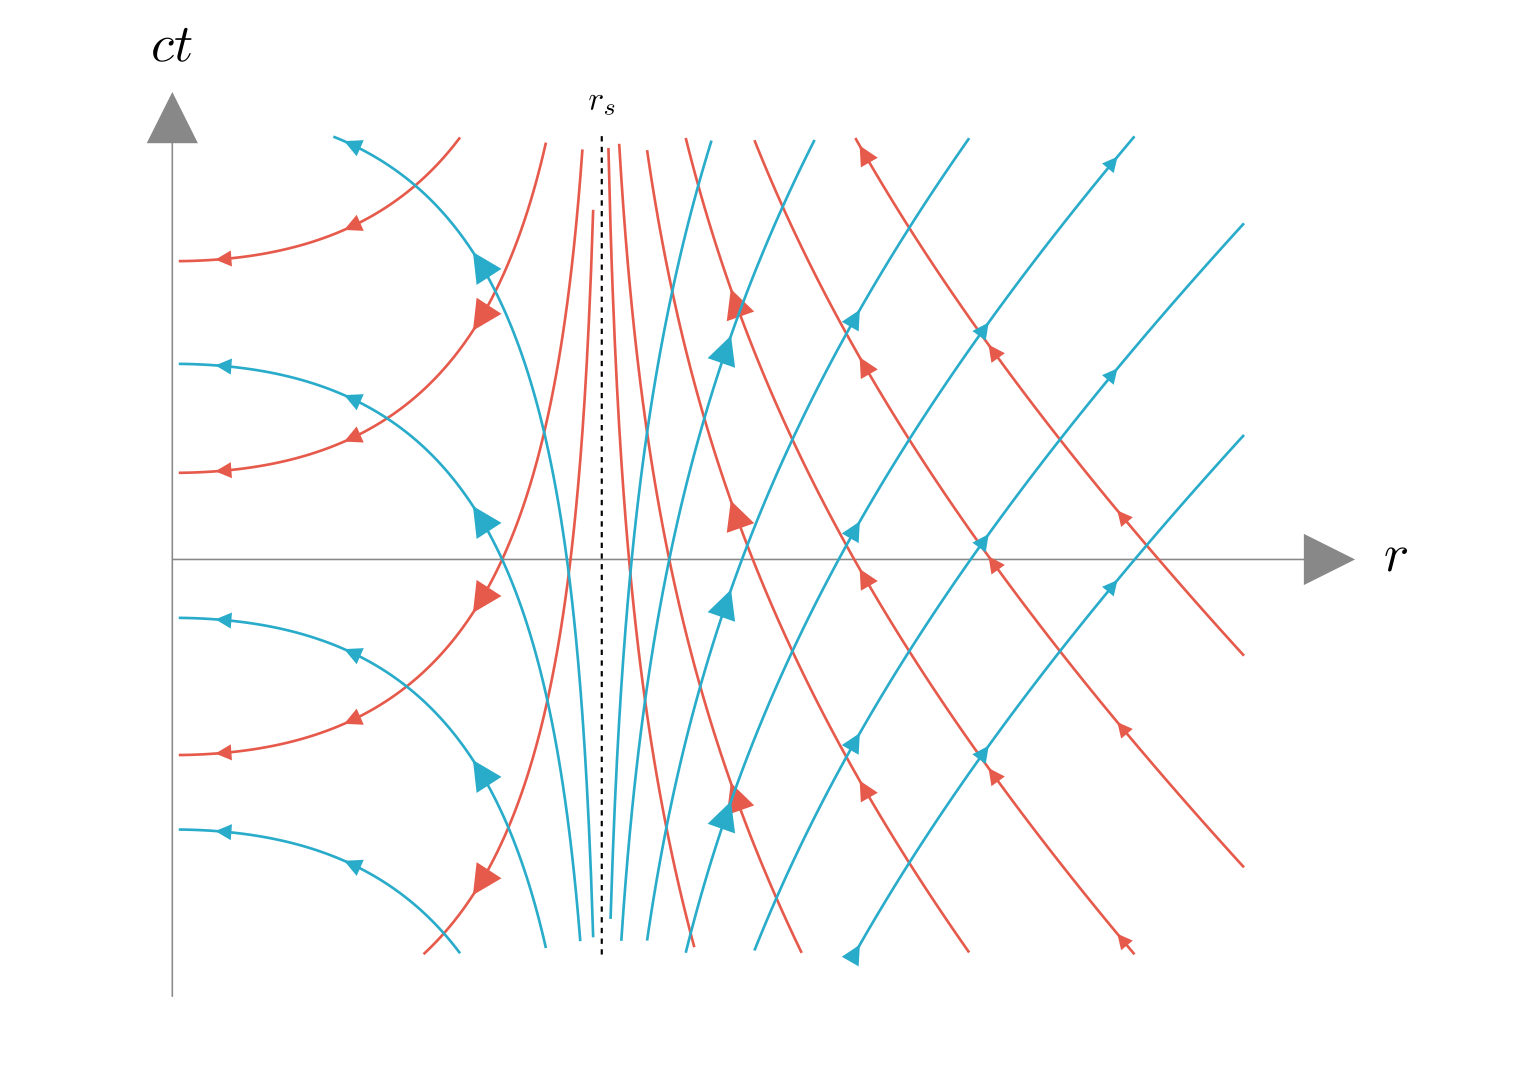
\includegraphics[width=0.95\textwidth]{AgujerosNegros/Schwarzschild/media/images/rayos_Luz_Schwarzschild_ManimCE_v0.19.0.png}
        \end{center}
        \caption{}
        \label{fig:lightraysSchwarzschild}
    \end{small}
\end{figure}

\subsection{ordenadas Eddington-Finkelstein}
Las coordenadas de Eddington-Finkelstein son un sistema de coordenadas para la solución de Schwarzschild cuya idea principal es usar las trayectorias de la luz (geodésicas nulas radiales) para definir las coordenadas temporal y radial. Esto es posible debido a la simetría radial, donde \( \theta, \varphi = \text{cte} \implies d\Omega^2 = 0 \).
Partimos de la trayectoria de la luz en términos de la coordenada radial \( r \) y el tiempo \( ct \):
\begin{equation}
    ct(r) = \pm \left( r + r_s \log \left| \frac{r}{r_s} - 1 \right| \right) + k,
\end{equation}
donde el signo \( + \) corresponde a geodésicas salientes y \( - \) a entrantes. Introducimos las nuevas variables \( c\tilde{t} \) y \( \tilde{r} \):
\begin{equation}
    \begin{aligned}
        c\tilde{t} & = ct + r_s \log \left| \frac{r}{r_s} - 1 \right|,         \\
        ct         & = c\tilde{t} - r_s \log \left| \frac{r}{r_s} - 1 \right|.
    \end{aligned}
\end{equation}
Combinando con la ecuación de las geodésicas entrantes (\( - \)):
\begin{equation}
    c\tilde{t} - r_s \log \left| \frac{r}{r_s} - 1 \right| = -r - r_s \log \left| \frac{r}{r_s} - 1 \right| + k,
\end{equation}
simplificando y renombrando la variable $\tilde{t} \to t$:
\begin{equation}
    c\tilde{t} = -r + k \to ct= -r + k .
\end{equation}
nos da las trayectorias de la luz entrantes al agujero negro.
Introducimos la coordenada \( v \):
\begin{equation}
    \begin{aligned}
        v  & = ct + r + r_s \log \left| \frac{r}{r_s} - 1 \right|, \\
        ct & = v - r - r_s \log \left| \frac{r}{r_s} - 1 \right|.
    \end{aligned}
\end{equation}
Reemplazando en la ecuación de los rayos de luz entrantes
\begin{equation}
    \begin{aligned}
        ct =v - r - r_s \log \left| \frac{r}{r_s} - 1 \right|  = - r - r_s \log \left| \frac{r}{r_s} - 1 \right| + k,
        v = k
    \end{aligned}
\end{equation}
y para los salientes
\begin{equation}
    \begin{aligned}
        ct = v - r - r_s \log \left| \frac{r}{r_s} - 1 \right|= r + r_s \log \left| \frac{r}{r_s} - 1 \right| + k, \\
        v = 2 \left(r_s \log \left| \frac{r}{r_s} - 1 \right|\right) +k
    \end{aligned}
\end{equation}
\begin{task}{Graficar}{}
    Gráfica esto.
\end{task}
Las coordenadas finales son:
\begin{equation}
    \boxed{
        v = ct + r + r_s \log \left| \frac{r}{r_s} - 1 \right|, \quad
        r_{\text{in}} = r
    }
\end{equation}

\subsubsection{Métrica de Schwarzschild en coordenadas de Eddington-Finkelstein}
La métrica se obtiene expresando los vectores base \( e_v \) y \( e_{r_{\text{in}}} \) en términos de las bases originales \( e_{ct} \) y \( e_r \). Primero, definimos \( r^* = r + r_s \log \left| \frac{r}{r_s} - 1 \right| \), con lo que:
\begin{equation}
    v = ct + r^*, \quad r_{\text{in}} = r.
\end{equation}

Las derivadas parciales para los vectores base son:
\begin{equation}
    \begin{aligned}
        e_v               & = \frac{\partial ct}{\partial v} e_{ct} + \frac{\partial r}{\partial v} e_r = e_{ct},                                                            \\
        e_{r_{\text{in}}} & = \frac{\partial ct}{\partial r_{\text{in}}} e_{ct} + \frac{\partial r}{\partial r_{\text{in}}} e_r = -\frac{1}{1 - \frac{r_s}{r}} e_{ct} + e_r.
    \end{aligned}
\end{equation}

Calculando \( \frac{dr^*}{dr} \):
\begin{equation}
    \frac{dr^*}{dr} = 1 + \frac{r_s}{r - r_s} = \frac{1}{1 - \frac{r_s}{r}}.
\end{equation}

Los componentes de la métrica \( g_{\mu\nu} = e_\mu \cdot e_\nu \) son:
\begin{equation}
    \begin{aligned}
        g_{vv}          & = e_v \cdot e_v = -\left(1 - \frac{r_s}{r}\right), \\
        g_{vr} = g_{rv} & = e_v \cdot e_{r_{\text{in}}} = 1,                 \\
        g_{rr}          & = e_{r_{\text{in}}} \cdot e_{r_{\text{in}}} = 0.
    \end{aligned}
\end{equation}
Por lo tanto, la métrica en coordenadas de Eddington-Finkelstein es:
\begin{equation}
    ds^2 = -\left(1 - \frac{r_s}{r}\right) dv^2 + 2 dv dr + r^2 d\Omega^2.
\end{equation}
\subsubsection{Coordenadas salientes de Eddington-Finkelstein}
Para geodésicas nulas salientes (\(+\)), partimos de:
\begin{equation}
    ct(r) = r + r_s \log \left| \frac{r}{r_s} - 1 \right| + k.
\end{equation}
Introducimos la coordenada \( u \):
\begin{equation}
    \begin{aligned}
        u  & = ct - r - r_s \log \left| \frac{r}{r_s} - 1 \right|, \\
        ct & = u + r + r_s \log \left| \frac{r}{r_s} - 1 \right|.
    \end{aligned}
\end{equation}
Para rayos salientes (\(+\)):
\begin{equation}
    \begin{aligned}
        u + r + r_s \log \left| \frac{r}{r_s} - 1 \right| = r + r_s \log \left| \frac{r}{r_s} - 1 \right| + k, \\
        u = k.
    \end{aligned}
\end{equation}
Y para los entrantes (\(-\)):
\begin{equation}
    \begin{aligned}
        u + r + r_s \log \left| \frac{r}{r_s} - 1 \right| = -r - r_s \log \left| \frac{r}{r_s} - 1 \right| + k, \\
        u = -2\left(r + r_s \log \left| \frac{r}{r_s} - 1 \right|  \right) +k.
    \end{aligned}
\end{equation}
\begin{task}{Graficar}{}
    Gráfica esto.
\end{task}
Las coordenadas finales son:
\begin{equation}
    \boxed{u = ct - r - r_s \log \left| \frac{r}{r_s} - 1 \right|, \quad r_{\text{out}} = r}.
\end{equation}

\subsubsection{Métrica en coordenadas salientes}

Definiendo \( r^* = r + r_s \log \left| \frac{r}{r_s} - 1 \right| \), tenemos:
\begin{equation}
    u = ct - r^*, \quad r_{\text{out}} = r.
\end{equation}

Vectores base en términos de \( e_{ct} \) y \( e_r \):
\begin{equation}
    \begin{aligned}
        e_u                & = \frac{\partial ct}{\partial u} e_{ct} + \frac{\partial r}{\partial u} e_r = e_{ct},                                                             \\
        e_{r_{\text{out}}} & = \frac{\partial ct}{\partial r_{\text{out}}} e_{ct} + \frac{\partial r}{\partial r_{\text{out}}} e_r = \frac{1}{1 - \frac{r_s}{r}} e_{ct} + e_r.
    \end{aligned}
\end{equation}

Componentes de la métrica \( g_{\mu\nu} = e_\mu \cdot e_\nu \):
\begin{equation}
    \begin{aligned}
        g_{uu}          & = e_u \cdot e_u = -\left(1 - \frac{r_s}{r}\right), \\
        g_{ur} = g_{ru} & = e_u \cdot e_{r_{\text{out}}} = -1,               \\
        g_{rr}          & = e_{r_{\text{out}}} \cdot e_{r_{\text{out}}} = 0.
    \end{aligned}
\end{equation}

La métrica en coordenadas salientes es:
\begin{equation}
    ds^2 = -\left(1 - \frac{r_s}{r}\right) du^2 - 2 du dr + r^2 d\Omega^2.
\end{equation}


En estas coordenadas:
\begin{itemize}
    \item Líneas con \( u = \text{cte} \) son geodésicas salientes con pendiente \( +1 \) en diagramas espacio-temporales.
    \item La métrica es regular en \( r = r_s \), eliminando la singularidad coordenada de Schwarzschild.
    \item \( r_{\text{out}} \) coincide con la coordenada radial areal.
\end{itemize}
\begin{itemize}
    \item Mostrar que las partículas de luz/masivas pueden pasar a través del horizonte de eventos, pero...
    \item En coordenadas de EF entrantes: los haces de luz salientes no funcionan en $r_s$
    \item En coordenadas de EF salientes: los haces de luz entrantes no funcionan en $r_s$
\end{itemize}


\subsection{Coordenadas Kruskal-Szekeres}

\subsubsection{Coordenadas nulas originales}
Definimos las coordenadas entrante (\(v\)) y saliente (\(u\)) de Eddington-Finkelstein:
\begin{equation}
    \begin{aligned}
        v   & = ct + r^*                                      \\
        u   & = ct - r^*                                      \\
        r^* & \equiv r + r_s \log\left|\frac{r}{r_s}-1\right|
    \end{aligned}
\end{equation}

\subsubsection{Vectores base en coordenadas \( (u, v) \)}
Expresamos los vectores base en términos de \( e_{ct} \) y \( e_r \):
\begin{equation}
    \begin{aligned}
        e_v & = \frac{\partial ct}{\partial v}e_{ct} + \frac{\partial r}{\partial v}e_r = \frac{1}{2}e_{ct} + \frac{1}{2}\left(1-\frac{r_s}{r}\right)^{-1}e_r \\
        e_u & = \frac{\partial ct}{\partial u}e_{ct} + \frac{\partial r}{\partial u}e_r = \frac{1}{2}e_{ct} - \frac{1}{2}\left(1-\frac{r_s}{r}\right)^{-1}e_r
    \end{aligned}
\end{equation}

\subsubsection{Productos punto fundamentales}
Usando la métrica de Schwarzschild \( g(e_{ct},e_{ct}) = -\left(1-\frac{r_s}{r}\right) \) y \( g(e_r,e_r) = \left(1-\frac{r_s}{r}\right)^{-1} \):
\begin{equation}
    \begin{aligned}
        e_v \cdot e_v & = \left(\frac{1}{2}\right)^2 g(e_{ct},e_{ct}) + \left(\frac{1}{2}\left(1-\frac{r_s}{r}\right)^{-1}\right)^2 g(e_r,e_r) = 0                                        \\
        e_u \cdot e_u & = \left(\frac{1}{2}\right)^2 g(e_{ct},e_{ct}) + \left(\frac{1}{2}\left(1-\frac{r_s}{r}\right)^{-1}\right)^2 g(e_r,e_r) = 0                                        \\
        e_v \cdot e_u & = \left(\frac{1}{2}\right)^2 g(e_{ct},e_{ct}) - \left(\frac{1}{2}\left(1-\frac{r_s}{r}\right)^{-1}\right)^2 g(e_r,e_r) = -\frac{1}{2}\left(1-\frac{r_s}{r}\right)
    \end{aligned}
\end{equation}

\subsubsection{Métrica en coordenadas nulas}
La métrica se expresa como:
\begin{equation}
    ds^2 = 2(e_v \cdot e_u) du\, dv + r^2 d\Omega^2 = -\left(1-\frac{r_s}{r}\right) du\, dv + r^2(d\theta^2 + \sin^2\theta d\varphi^2)
\end{equation}

\subsubsection{Transformación a Kruskal-Szekeres}

\begin{equation}
    \begin{aligned}
        \frac{v-u}{2}=r+r_s \log \left|\frac{r}{r_s}-1\right|                 \\
        \frac{v-u}{2 r_s}=\frac{r}{r_s}+\log \left|\frac{r}{r_s}-1\right|     \\
        e^{\frac{v-u}{2 r_s}}=e^{\frac{r}{r_s}+\log \abs{ \frac{r}{r_s} 1} }, \\
        -e^{\frac{v}{2 r_s}}\left(-e^{-\frac{u}{2 r_s}}\right)=e^{\frac{r}{r_s}}\left|\frac{r}{r_s}-1\right|
    \end{aligned}
\end{equation}
Definimos las nuevas coordenadas:
\begin{equation}
    \mathcal{U} = -e^{-\frac{u}{4r_s}}, \quad \mathcal{V} = e^{\frac{v}{4r_s}}
\end{equation}

\subsubsection{Vectores base en Kruskal-Szekeres}
Relación diferencial usando la regla de la cadena:
\begin{equation}
    \begin{aligned}
        e_\mathcal{U} & = \frac{\partial u}{\partial \mathcal{U}} e_u = 4r_s e^{\frac{u}{4r_s}} e_u = -4r_s \mathcal{U}^{-1} e_u \\
        e_\mathcal{V} & = \frac{\partial v}{\partial \mathcal{V}} e_v = 4r_s e^{-\frac{v}{4r_s}} e_v = 4r_s \mathcal{V}^{-1} e_v
    \end{aligned}
\end{equation}

\subsubsection{Producto punto clave}
Calculamos el producto punto usando \( e_u \cdot e_v = -\frac{1}{2}\left(1-\frac{r_s}{r}\right) \):
\begin{equation}
    e_\mathcal{U} \cdot e_\mathcal{V} = (-4r_s \mathcal{U}^{-1})(4r_s \mathcal{V}^{-1})(e_u \cdot e_v) = \frac{8r_s^2}{\mathcal{U}\mathcal{V}}\left(1-\frac{r_s}{r}\right)
\end{equation}

\subsubsection{Relación geométrica fundamental}
De la definición de \( \mathcal{U} \) y \( \mathcal{V} \):
\begin{equation}
    \mathcal{U}\mathcal{V} = -e^{\frac{r^*}{2r_s}} = -\left|\frac{r}{r_s}-1\right|^{1/2}e^{\frac{r}{2r_s}}
\end{equation}

Sustituyendo en el producto punto:
\begin{equation}
    e_\mathcal{U} \cdot e_\mathcal{V} = \frac{32r_s^3}{r}e^{-\frac{r}{r_s}}
\end{equation}

\subsubsection{Métrica final de Kruskal-Szekeres}
La métrica toma su forma canónica:
\begin{equation}
    \boxed{ds^2 = \frac{32r_s^3}{r}e^{-\frac{r}{r_s}} d\mathcal{U}d\mathcal{V} + r^2(d\theta^2 + \sin^2\theta d\varphi^2)}
\end{equation}

\begin{equation}
    \text{con } \mathcal{U}\mathcal{V} = \left(1-\frac{r}{r_s}\right)e^{\frac{r}{r_s}} \quad \text{y} \quad \frac{\mathcal{V}}{\mathcal{U}} = -e^{\frac{ct}{2r_s}}
\end{equation}
De momento $\mathcal{V}$ y $\mathcal{U}$ son coordenadas nulas, que describen trayectorias de luz, pero podemos hacerlas espaciales y temporales definiendo:
\begin{equation}
    \begin{aligned}
        T \equiv \frac{\mathcal{V}+\mathcal{U}}{2} \\
        X \equiv \frac{\mathcal{V}-\mathcal{U}}{2} \\
    \end{aligned}
\end{equation}
y viceversa
\begin{equation}
    \begin{aligned}
        \mathcal{V}=T+X \\
        \mathcal{U}=T-X
    \end{aligned}
\end{equation}
De modo que la métrica en términos de $T$ y $X$ es:
\begin{equation}
        g_{\mu \nu} =\left[\begin{array}{cccc}
                                             +\frac{4 r_s^3}{r} e^{-\frac{r}{r_s}} & 0                                     & 0    & 0                   \\
                                             0                                     & -\frac{4 r_s^3}{r} e^{-\frac{r}{r_s}} & 0    & 0                   \\
                                             0                                     & 0                                     & -r^2 & 0                   \\
                                             0                                     & 0                                     & 0    & -r^2(\sin \theta)^2
                                         \end{array}\right]
\end{equation}
Usando el mismo truco que usamos anteriormente podemos encontar las geodésicas nulas en estas coordenadas.
\begin{equation}
    \begin{array}{l}
        0=\left(\frac{d T}{d \lambda}\right)^2\left(\frac{\partial}{\partial T} \cdot \frac{\partial}{\partial T}\right)+\left(\frac{d X}{d \lambda}\right)^2\left(\frac{\partial}{\partial X} \cdot \frac{\partial}{\partial X}\right) \\
        0=\left(\frac{d T}{d \lambda}\right)^2 g_{T T}+\left(\frac{d X}{d \lambda}\right)^2 g_{X X}                                                                                                                                     \\
        0=\left(\frac{d T}{d \lambda}\right)^2\left(+2 g_{U V}\right)+\left(\frac{d X}{d \lambda}\right)^2\left(-2 g_{U V}\right)
    \end{array}
\end{equation}

\begin{equation}
    \d{X}{\lambda} =\pm \d{T}{\lambda} \to \d{X}{T} = \pm 1 \to T = \pm Y + k
\end{equation}

Eso quiere decir que las geodésicas nulas en estas coordenadas son rectas en el espacio-tiempo. 
ahora volver a poner las coordenadas en términos de $r$ y $t$ solo es cuestión de una composición de funciones.

\begin{equation}
    \begin{aligned}
        T&=\frac{V+U}{2} \\
        X&=\frac{V-U}{2}
    \end{aligned}
    \quad ; 
    \begin{aligned}
        V&=e^{\frac{v}{2 r_s}} \\
        U&=-e^{-\frac{u}{2 r_s}}
    \end{aligned}
    \quad ; 
    \begin{aligned}
        v&=c t+r+r_s \log \left|\frac{r}{r_s}-1\right| \\
        u&=c t-r-r_s \log \left|\frac{r}{r_s}-1\right|
    \end{aligned}
\end{equation}
Simplificando
\begin{equation}
    \begin{aligned}
        T & =  \frac{1}{2}\left(V + U\right)                                                                                                                                                      \\
          & = \frac{1}{2} e^{\frac{v}{2 r_s}}-\frac{1}{2} e^{-\frac{u}{2 r_S}}                                                                                                                    \\
          & = \frac{1}{2} e^{\frac{1}{2 r_s}\left(c t+r+r_s \log \left|\frac{r}{r_s}-1\right|\right)}-\frac{1}{2} e^{-\frac{1}{2 r_s}\left(c t-r-r_s \log \left|\frac{r}{r_s}-1\right|\right)}    \\
          & =\frac{1}{2} e^{\frac{c t}{2 r_s}} e^{\frac{r}{2 r_s}}\left(\left|\frac{r}{r_s}-1\right|\right)^{1 / 2}-\frac{1}{2} e^{\frac{-c t}{2 r_s}} e^{\frac{r}{2 r_s}}\left(\left|\frac{r}{r_s}-1\right|\right)^{1 / 2} \\
          & = e^{\frac{r}{2 r_s}} \sqrt{\left|\frac{r}{r_s}-1\right|} \frac{1}{2}\left(e^{\frac{c t}{2 r_s}}-e^{\frac{-c t}{2 r_s}}\right)                                                                     \\
          & = e^{\frac{r}{2 r_s}} \sqrt{\left|\frac{r}{r_s}-1\right|} \sinh\left(\frac{ct}{2r_s}\right)
          \label{eq:Kruskal-SzekeresT(r,t)}
    \end{aligned}
\end{equation}
y para $X$ el calculo es prácticamente el mismo a excepción de un signo ($+$) en la diferencia de exponentes.
\begin{equation}
        X  = e^{\frac{r}{2 r_s}} \sqrt{\left|\frac{r}{r_s}-1\right|}  \cosh\left(\frac{ct}{2r_s}\right)
        \label{eq:Kruskal-SzekeresX(r,t)}
\end{equation}
Donde podemos desarrollar la siguiente identidad
\begin{equation}
    \begin{aligned}
        T^2 - X^2 &= \left( e^{\frac{r}{2r_s}} \sqrt{\left|\frac{r}{r_s}-1\right|}\, \sinh\left(\frac{ct}{2r_s}\right) \right)^2 
        - \left( e^{\frac{r}{2r_s}} \sqrt{\left|\frac{r}{r_s}-1\right|}\, \cosh\left(\frac{ct}{2r_s}\right) \right)^2\\[1mm]
        &= e^{\frac{r}{r_s}} \left|\frac{r}{r_s}-1\right| \left[ \sinh^2\left(\frac{ct}{2r_s}\right) - \cosh^2\left(\frac{ct}{2r_s}\right) \right]\\[1mm]
        &= -\, e^{\frac{r}{r_s}} \left|\frac{r}{r_s}-1\right|\\[2mm]
        &=
        \begin{cases}
            -\, e^{\frac{r}{r_s}} \left(\dfrac{r}{r_s}-1\right), & \text{si } r > r_s,\\[2mm]
            -\, e^{\frac{r}{r_s}} \left(1-\dfrac{r}{r_s}\right), & \text{si } r < r_s.
        \end{cases}
    \end{aligned}
    \label{eq:Kruskal-SzekeresT^2-X^2}
\end{equation}
\begin{task}{Demostrar}{}
    Demostrar la identidad (\ref{eq:Kruskal-SzekeresT^2-X^2}).
\end{task}
Esta identidad nos ayuda a determinar las líneas de \(r\) constante en el espacio-tiempo de Schwarzschild. Lo interesante ocurre cuando observamos el caso \(r < r_s\): el valor absoluto \(\left|\frac{r}{r_s}-1\right|\) en la ecuación (\ref{eq:Kruskal-SzekeresT^2-X^2}) se puede expresar como \(1-\frac{r}{r_s}\). ¿Por qué es importante notar esto? Si nos fijamos en la segunda línea de la ecuación, podemos identificar los coeficientes de la siguiente forma:
\begin{equation}
    \begin{aligned}
        T^2 - X^2 &= e^{\frac{r}{r_s}} \left(1-\frac{r}{r_s}\right) \left[ \sinh^2\left(\frac{ct}{2r_s}\right) - \cosh^2\left(\frac{ct}{2r_s}\right) \right] \\
        &= -\, e^{\frac{r}{r_s}} \left(\frac{r}{r_s}-1\right) \left[ \sinh^2\left(\frac{ct}{2r_s}\right) - \cosh^2\left(\frac{ct}{2r_s}\right) \right] \\
        &= e^{\frac{r}{r_s}} \left(\frac{r}{r_s}-1\right) \left[ \cosh^2\left(\frac{ct}{2r_s}\right) - \sinh^2\left(\frac{ct}{2r_s}\right) \right].
    \end{aligned}
\end{equation}
De ello se deduce que, dentro del horizonte de eventos (\(r < r_s\)), se tienen las siguientes expresiones:
\begin{equation}
    X = e^{\frac{r}{2r_s}} \sqrt{1-\frac{r}{r_s}} \, \frac{1}{2} \sinh\left(\frac{ct}{2r_s}\right), \quad 
    T = e^{\frac{r}{2r_s}} \sqrt{1-\frac{r}{r_s}} \, \frac{1}{2} \cosh\left(\frac{ct}{2r_s}\right).
\end{equation}
Dado que el negativo de estas coordenadas $-X$ y $-T$ cumplen la identidad (\ref{eq:Kruskal-SzekeresT^2-X^2}) podemos escribir lo que se llama la extensión máxima de las coordenadas de Kruskal-Szekeres
\begin{table}[H]
    \centering
    \caption{Extensión máxima de las coordenadas de Kruskal-Szekeres}
    \begin{tabular}{|c|c|c|}
        \hline Region & $T$                                                                                         & $X$                                                                                \\
        \hline$I$        & $+\sinh \left(\frac{c t}{2 r_s}\right)\frac{r}{2 r_s} \sqrt{\frac{r}{r_s}-1}$ & $+\cosh \left(\frac{c t}{2 r_s}\right) e^{\frac{r}{2 r_s}} \sqrt{\frac{r}{r_s}-1}$ \\
        \hline$I I$       & $+\cosh \left(\frac{c t}{2 r_s}\right) e^{\frac{r}{2 r_s}} \sqrt{1-\frac{r}{r_s}}$          & $+\sinh \left(\frac{c t}{2 r_s}\right) e^{\frac{r}{2 r_s}} \sqrt{1-\frac{r}{r_s}}$ \\
        \hline$I I I$   & $-\sinh \left(\frac{c t}{2 r_s}\right) e^{\frac{r}{2 r_s}} \sqrt{\frac{r}{r_s}-1}$          & $-\cosh \left(\frac{c t}{2 r_s}\right) e^{\frac{r}{2 r_s}} \sqrt{\frac{r}{r_s}-1}$ \\
        \hline$I V$      & $-\cosh \left(\frac{c t}{2 r_s}\right) e^{\frac{r}{2 r_s}} \sqrt{1-\frac{r}{r_s}}$          & $-\sinh \left(\frac{c t}{2 r_s}\right) e^{\frac{r}{2 r_s}} \sqrt{1-\frac{r}{r_s}}$ \\
        \hline
    \end{tabular}
\end{table}
Ahora para la lineas de tiempo constante es fácil ver la siguiente relación
\begin{equation}
    \tanh \left(\frac{ct}{2 r_s}\right)=\left\{\begin{array}{ll}
        T / X & \text { (en region I y III) } \\
        X / T & \text { (en region II y IV) }
        \end{array}\right.
\end{equation}
Con esto tenemos todo lo necesario para construir el diagrama de Kruskal-Szekeres.  
\begin{figure}[H]
    \begin{small}
        \begin{center}
            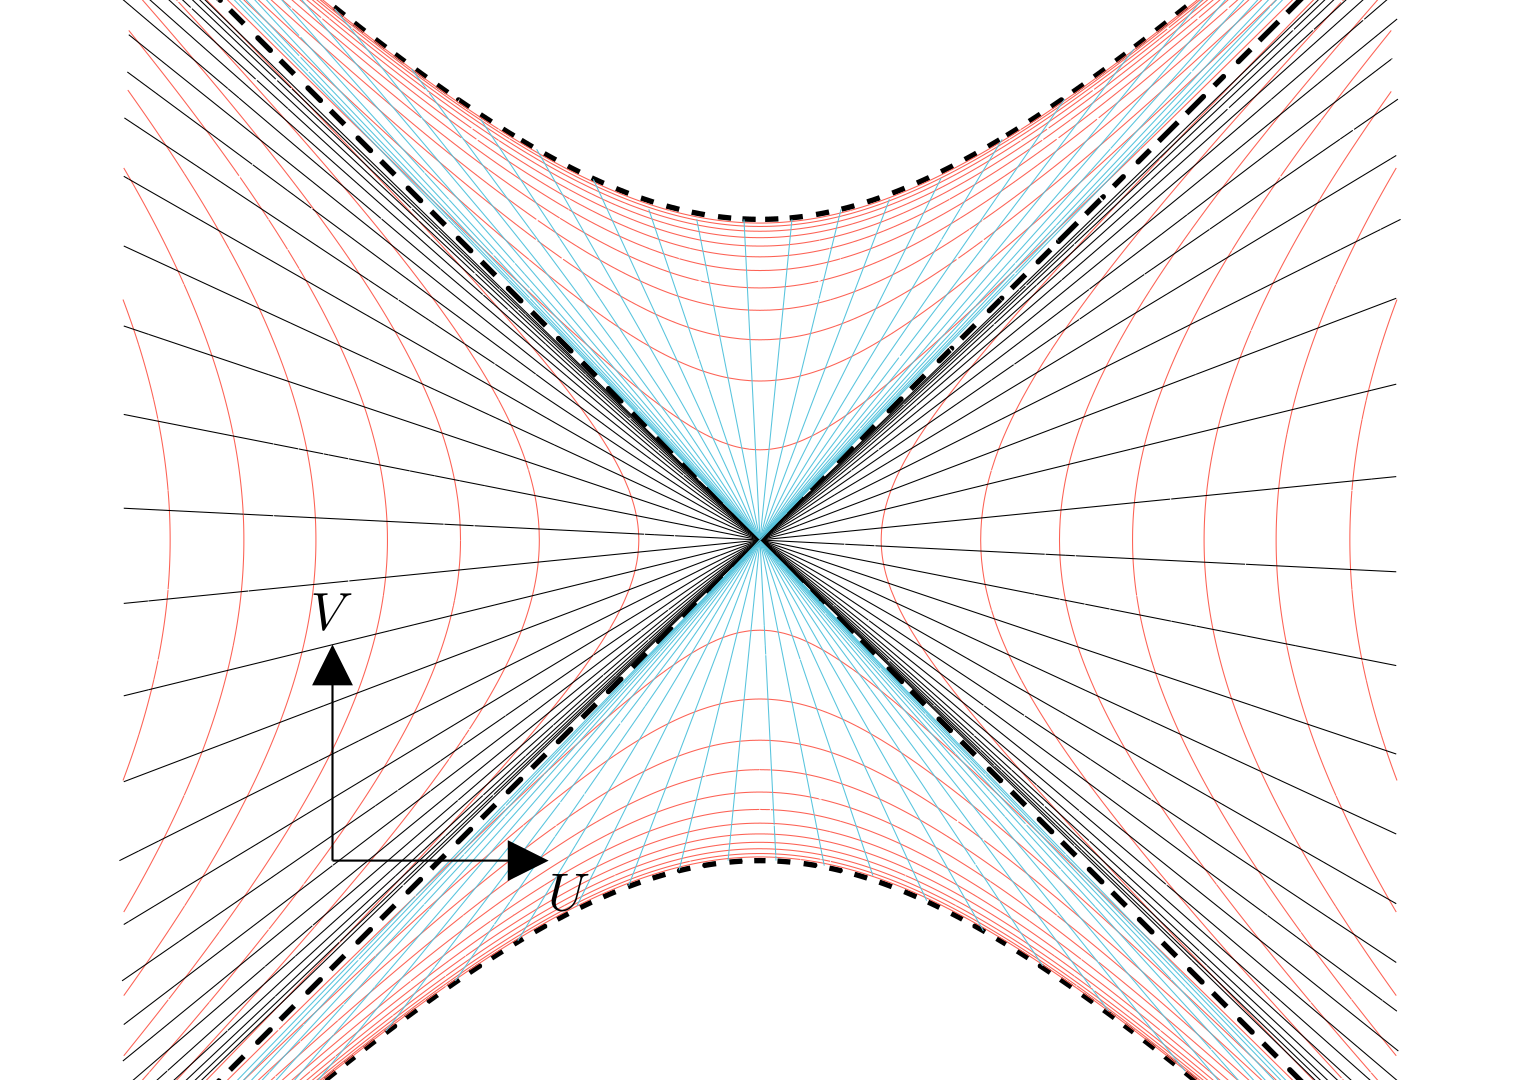
\includegraphics[width=0.95\textwidth]{AgujerosNegros/Schwarzschild/media/images/Kruskal_Szekeres_diagram_ManimCE_v0.19.0.png}
        \end{center}
        \caption{}
        \label{fig:}
    \end{small}
\end{figure}

\section{Diagramas de Penrose y estructura causal.}

\section{Algoritmo de Newman-Janis y agujeros negros rotantes}

El algoritmo de Newman-Janis es una técnica en relatividad general que permite generar soluciones exactas a las ecuaciones de Einstein. En 1965, Ezra T. Newman y Alfred I. Janis \cite{newman-1965} descubrieron que, mediante una transformación de coordenadas complejas aplicada a la métrica de Schwarzschild, podían obtener la métrica de Kerr, que describe un agujero negro en rotación.

Particularmente nos centraremos en usar el desarrollo hecho por \cite{drake-2000} donde da una versión de este algoritmo donde remueve algunas de las ambigüedades presentes en el trabajo original de \cite{newman-1965}.

El algoritmo se puede resumir en 5 pasos:

\begin{enumerate}[1.]
    \item Escribe un elemento de línea estático y esféricamente simétrico en coordenadas nulas avanzadas $\{u, r, \theta, \phi\}$:

          \begin{equation}
              ds^2 = e^{2 \Phi(r)} du^2 + e^{\Phi(r) + \lambda(r)} du dr - r^2 (d\theta^2 + \sin^2 \theta d\phi^2)
          \end{equation}

    \item Expresar la forma contravariante de la métrica en términos de un tetrad nulo:

          \begin{equation}
              g^{\mu \nu} = l^\mu n^\nu + l^\nu n^\mu - m^\mu \bar{m}^\nu - m^\nu \bar{m}^\mu
              \label{MetricaTetrada}
          \end{equation}

          donde

          \begin{equation}
              l_\mu l^\mu = m_\mu m^\mu = n_\mu n^\mu = 0, \quad l_\mu n^\mu = -m_\mu \bar{m}^\mu = 1, \quad l_\mu m^\mu = n_\mu m^\mu = 0
          \end{equation}

          Donde los tetrads nulos tendrán la forma inicial:

          \begin{equation}
              \begin{aligned}
                  l^\mu & = \delta_1^\mu                                                                          \\
                  n^\mu & = e^{-\lambda(r) - \Phi(r)} \delta_0^\mu - \frac{1}{2} e^{-2 \lambda(r)} \delta_1^\mu   \\
                  m^\mu & = \frac{1}{\sqrt{2} r} \left( \delta_2^\mu + \frac{i}{\sin \theta} \delta_3^\mu \right)
              \end{aligned}
          \end{equation}

          En este punto es conveniente usar la notación de tetradas:

          \begin{equation}
              Z_a^\mu = (l^\mu, n^\mu, m^\mu, \bar{m}^\mu), \quad a = 1, 2, 3, 4
          \end{equation}

    \item El siguiente paso es hacer una transformación compleja directa que extiende las coordenadas $x^\rho$ a un nuevo conjunto de coordenadas complejas $\tilde{x}^\rho$:

          \begin{equation}
              x^\rho \rightarrow \tilde{x}^\rho = x^\rho + i y^\rho(x^\sigma)
          \end{equation}

          donde $y^\rho(x^\sigma)$ son funciones analíticas de las coordenadas reales $x^\sigma$, y simultáneamente dejamos que los vectores tetrad nulos $Z_a^\mu$ sufran una transformación:

          \begin{equation}
              Z_a^\mu(x^\rho) \rightarrow \tilde{Z}_a^\mu(\tilde{x}^\rho, \overline{\tilde{x}}^\rho)
          \end{equation}

          Finalmente requerimos como condición que la transformación recupere el tetrad y la métrica antiguos cuando $\tilde{x}^\rho = \overline{\tilde{x}}^\rho$. En resumen, el efecto de esta "transformación tilde" es crear una nueva métrica cuyos componentes (reales) son funciones de variables complejas:

          \begin{equation}
              g_{\mu \nu} \rightarrow \tilde{g}_{\mu \nu}: \tilde{x} \times \tilde{x} \mapsto \mathbb{R}
          \end{equation}

          mientras que se debe de cumplir también:

          \begin{equation}
              \left. \tilde{Z}_a^\mu(\tilde{x}^\rho, \overline{\tilde{x}}^\rho) \right|_{\overline{x} = \tilde{x}} = Z_a^\mu(x^\rho)
          \end{equation}

          La transformación tilde claramente no es única, ya que existen muchas opciones diferentes para los coeficientes de los vectores tetrad nulos que satisfacen las condiciones. En el paper original \cite{newman-1965} se elige la transformación tilde como:

          \begin{equation}
              \tilde{x}^\rho = x^\rho + i a \cos x^2 (\delta_0^\rho - \delta_1^\rho) = x^\rho + i a \cos \theta (\delta_0^\rho - \delta_1^\rho)
          \end{equation}

          En este caso, la transformación tilde se escribe para cada coordenada $\rho$ como:

          \begin{itemize}
              \item Para $\rho = 0$ (coordenada $u$):
                    \begin{equation}
                        \tilde{u} = u + i a \cos \theta
                    \end{equation}
                    porque $\delta_0^0 = 1$ y $\delta_1^0 = 0$.

              \item Para $\rho = 1$ (coordenada $r$):
                    \begin{equation}
                        \tilde{r} = r - i a \cos \theta
                    \end{equation}
                    ya que $\delta_0^1 = 0$ y $\delta_1^1 = 1$.

              \item Para $\rho = 2, 3$ (coordenadas $\theta$ y $\phi$):
                    \begin{equation}
                        \tilde{\theta} = \theta, \quad \tilde{\phi} = \phi
                    \end{equation}
                    pues $\delta_0^\rho - \delta_1^\rho = 0$ para $\rho = 2, 3$.
          \end{itemize}

          Después de aplicar la transformación, las coordenadas $\tilde{x}^\rho$ son complejas. El radio $r$ se reemplaza por $\tilde{r} = r - i a \cos \theta$, lo que permitirá que las funciones métricas (por ejemplo, $e^{2 \Phi}$) pasen a tener una dependencia combinada en $r$ y $\theta$.

          \begin{itemize}
              \item $u \rightarrow \tilde{u} = u + ia \cos \theta$ (coordenada tipo luz)
              \item $r \rightarrow \tilde{r} = r - i a \cos \theta$
              \item $\theta \rightarrow \tilde{\theta} = \theta$
              \item $\phi \rightarrow \tilde{\phi} = \phi$
          \end{itemize}

          \begin{equation}
              \begin{aligned}
                  l^\mu & \rightarrow \tilde{l}^\mu = \delta_1^\mu                                                                                                                                                                  \\
                  n^\mu & \rightarrow \tilde{n}^\mu = e^{-\lambda(\tilde{r}, \overline{\tilde{r}}) - \phi(\tilde{r}, \overline{\tilde{r}})} \delta_0^\mu - \frac{1}{2} e^{-2 \lambda(\tilde{r}, \overline{\tilde{r}})} \delta_1^\mu \\
                  m^\mu & \rightarrow \tilde{m}^\mu = \frac{1}{\sqrt{2} \overline{\tilde{r}}} \left( \delta_2^\mu + \frac{i}{\sin \tilde{\theta}} \delta_3^\mu \right)
              \end{aligned}
          \end{equation}

          En este paso se extiende la variable radial $r$ a una variable compleja. La idea es reemplazar $r$ por $\tilde{r}$ (y análogamente para $\theta$ si fuera necesario) de modo que las funciones métricas pasen a depender de dos variables: $r$ y $\theta$. De esta forma, se escriben las funciones como $\phi(\tilde{r}, \overline{\tilde{r}})$ y $\lambda(\tilde{r}, \overline{\tilde{r}})$.

          \begin{itemize}
              \item $\tilde{r} \rightarrow r$,
              \item $\overline{\tilde{r}} \rightarrow r$,
              \item $\tilde{\theta} \rightarrow \theta$,
              \item $\tilde{r} + \overline{\tilde{r}} = 2r$,
              \item $\tilde{r} - \overline{\tilde{r}} = 2ia \cos \theta$.
          \end{itemize}
          \begin{note}[Problema de la Complejidad]
              Una métrica compleja no tiene sentido físico en relatividad general, ya que el espacio-tiempo es real. Por lo tanto, se requiere eliminar las partes imaginarias introducidas por la complejificación. Esto se logra mediante la condición de realidad.

              \textbf{Mecanismo de la Condición de Realidad}

              La condición de realidad opera en dos niveles:
              \begin{enumerate}[a.]
                  \item \textbf{Sustitución de $\tilde{r}$ y $\overline{\tilde{r}}$}

                        Se reemplazan las combinaciones de $\tilde{r}$ (complejo) y su conjugado $\overline{\tilde{r}} = r - ia \cos \theta$ por expresiones reales que dependen de $r$ y $\theta$. Por ejemplo:

                        $$
                            \tilde{r} + \overline{\tilde{r}} = 2r, \quad \tilde{r} \overline{\tilde{r}} = r^2 + a^2 \cos^2 \theta.
                        $$

                        Ejemplo:
                        Si una función compleja es $f(\tilde{r}) = \frac{1}{\tilde{r}}$, la condición de realidad la convierte en:

                        $$
                            f(r, \theta) = \frac{1}{r^2 + a^2 \cos^2 \theta} \cdot (r - ia \cos \theta)
                        $$

                        pero solo se conserva la parte real relevante para la métrica.
                  \item  \textbf{Simetrización de Funciones}

                        Las funciones que dependían originalmente de $r$ en la métrica estática se redefinen como funciones simétricas en $\tilde{r}$ y $\overline{\tilde{r}}$. Por ejemplo:
                        - En la métrica de Schwarzschild, $1 - \frac{2M}{r}$ se convierte en $1 - \frac{2M}{\tilde{r}} \rightarrow 1 - \frac{2Mr}{r^2 + a^2 \cos^2 \theta}$.

              \end{enumerate}



              \textbf{Aplicación en las Tetradas}

              Las tetradas nulas $l^\mu, n^\mu, m^\mu$ también se afectan por la complejificación. Para garantizar su realidad:

              \begin{enumerate}[a.]
                  \item \textbf{Tetrada $m^\mu$}

                        La parte angular $m^\mu$ adquiere un término adicional $ia \sin \theta (\delta_0^\mu - \delta_1^\mu)$, que cancela las contribuciones imaginarias del denominador complejo $\tilde{r} = r + ia \cos \theta$.
                        Ejemplo:

                        $$
                            m^\mu = \frac{1}{\sqrt{2}(r + ia \cos \theta)} \left( ia \sin \theta (\delta_0^\mu - \delta_1^\mu) + \delta_2^\mu + \frac{i}{\sin \theta} \delta_3^\mu \right)
                        $$

                  \item \textbf{Tetradas $l^\mu$ y $n^\mu$}

                        Se mantienen reales al reemplazar $\tilde{r} \rightarrow r$ en sus componentes radiales, pero incorporando $a$ en las funciones $\phi(r, \theta)$ y $\lambda(r, \theta)$.
              \end{enumerate}
          \end{note}




    \item Se obtiene una nueva métrica al realizar una transformación de coordenadas complejas en los vectores tetrad nulos $\tilde{Z}_a^\mu$. Los vectores tetrad nulos se transforman de la manera habitual:

          \begin{equation}
              Z_a^\mu = \tilde{Z}_a^\nu \frac{\partial x^\mu}{\partial \tilde{x}^\nu}
          \end{equation}

          mediante esta transformación, de forma genérica podemos efectuar la de las tetradas $m^\mu = \tilde{m}^\nu \frac{\partial x^\mu}{\partial \tilde{x}^\nu}$ y $l^\mu = \tilde{l}^\nu \frac{\partial x^\mu}{\partial \tilde{x}^\nu}$:
          \begin{note}
            Las derivadas parciales $\pd{x^\mu}{\tilde{x}^\nu}$ las tomamos a partir de las transformaciones inversas:
            $$\begin{aligned} u & =\tilde{u}-i a \cos \tilde{\theta} \\ r & =\tilde{r}+i a \cos \tilde{\theta} \\ \theta & =\tilde{\theta} \\ \phi & =\tilde{\phi}\end{aligned}$$
            y la matriz jacobiana de la transformación es:
            \begin{equation}
               \left(\pd{x^\mu}{\tilde{x}^\nu}\right) =\left(\begin{array}{cccc}
                1 & 0 & +i a \sin \theta & 0\\
                0 & 1 & -i a \sin \theta & 0\\
                0 & 0 & 1 & 0\\
                0 & 0 & 0& 1
                \end{array}\right)
                \end{equation}
                Lo cual nos da que:
                \begin{align*}
                \pd{x^\mu}{\tilde{x}^0}&= \delta^\mu_0\\
                \pd{x^\mu}{\tilde{x}^1}&= \delta^\mu_1\\
                \pd{x^\mu}{\tilde{x}^2}&= ia (\delta^\mu_0 - \delta^\mu_1)\sin \theta + \delta^\mu_2\\
                \pd{x^\mu}{\tilde{x}^3}&=\delta^\mu_3
                \end{align*}
          \end{note}
          \begin{equation}
              \begin{aligned}
                  l^\mu & = \tilde{l}^\nu \frac{\partial x^\mu}{\partial \tilde{x}^\nu}                                                                                                                                                                           \\
                        & = \tilde{l}^0 \frac{\partial x^\mu}{\partial \tilde{x}^0} + \tilde{l}^1 \frac{\partial x^\mu}{\partial \tilde{x}^1} + \tilde{l}^2 \frac{\partial x^\mu}{\partial \tilde{x}^2} + \tilde{l}^3 \frac{\partial x^\mu}{\partial \tilde{x}^3} \\
                        & = \delta_1^0 \frac{\partial x^\mu}{\partial \tilde{x}^0} + \delta_1^1 \frac{\partial x^\mu}{\partial \tilde{x}^1} + \delta_1^2 \frac{\partial x^\mu}{\partial \tilde{x}^2} + \delta_1^3 \frac{\partial x^\mu}{\partial \tilde{x}^3}     \\
                        & = \delta_1^1 \frac{\partial x^\mu}{\partial \tilde{x}^1} = \delta_1^\mu
              \end{aligned}
          \end{equation}

          el caso $m^\mu = \tilde{m}^\nu \frac{\partial x^\mu}{\partial \tilde{x}^\nu}$:

          \begin{equation}
              \begin{aligned}
                  m^\mu & = \tilde{m}^\nu \frac{\partial x^\mu}{\partial \tilde{x}^\nu}                                                                                                                                                                                                                           \\
                        & = \tilde{m}^0 \frac{\partial x^\mu}{\partial \tilde{x}^0} + \tilde{m}^1 \frac{\partial x^\mu}{\partial \tilde{x}^1} + \tilde{m}^2 \frac{\partial x^\mu}{\partial \tilde{x}^2} + \tilde{m}^3 \frac{\partial x^\mu}{\partial \tilde{x}^3}                                                 \\
                        & = 0 * \frac{\partial x^\mu}{\partial \tilde{x}^0} + 0 * \frac{\partial x^\mu}{\partial \tilde{x}^1} + \frac{1}{\sqrt{2} \tilde{r}} \frac{\partial x^\mu}{\partial \tilde{x}^2} + \frac{1}{\sqrt{2} \tilde{r}} \frac{i}{\sin \tilde{\theta}} \frac{\partial x^\mu}{\partial \tilde{x}^3} \\
                        & = \frac{1}{\sqrt{2}(r + ia \cos \theta)} \left( ia \sin \theta (\delta_0^\mu - \delta_1^\mu) + \delta_2^\mu + \frac{i}{\sin \theta} \delta_3^\mu \right)
              \end{aligned}
          \end{equation}

          dado que la tetrada $n^\mu$ es particular para cada métrica semilla que se use, el cálculo de esta debe de hacerse de forma particular. Al efectuar la transformación del tetrad, se obtiene:

          \begin{equation}
              \begin{aligned}
                  l^\mu & = \delta_1^\mu     \\
                  m^\mu & = \frac{1}{\sqrt{2}(r + ia \cos \theta)} \left[ ia \sin \theta (\delta_0^\mu - \delta_1^\mu) + \delta_2^\mu + \frac{i}{\sin \theta} \delta_3^\mu \right]
              \end{aligned}
          \end{equation}

    \item \begin{task}
        Convertir la métrica obtenida a coordenadas de Boyer-Lindquist, que son las coordenadas más comunes para describir agujeros negros rotantes. 
    \end{task}
\end{enumerate}

\subsection{Aplicación a la métrica de Schwarzschild}
La métrica de Schwarzschild en coordenadas avanzadas de Eddington-Finkelstein es:
\begin{equation}
    ds^2=\left(1-\frac{2 m}{r}\right) d u^2+2 d u d r-r^2\left(d \theta^2+\sin ^2 \theta d \phi^2\right) .
\end{equation}

El "seed metric" propuesto es

\begin{equation}
    d s^2=e^{2 \Phi(r)} d u^2+e^{\Phi(r)+\lambda(r)} d u d r-r^2\left(d \theta^2+\sin ^2 \theta d \phi^2\right)
\end{equation}

Comparando término a término con la métrica obtenida:
Tenemos

\begin{equation}
    e^{2 \Phi(r)}=1-\frac{2 m}{r}
\end{equation}

lo que implica

\begin{equation}
    \Phi(r)=\frac{1}{2} \ln \left(1-\frac{2 M}{r}\right) .
\end{equation}

En la métrica obtenida aparece el coeficiente +2 , por lo que se identifica

\begin{equation}
    e^{\Phi(r)+\lambda(r)}=2
\end{equation}

Despejando para $\lambda(r)$,

\begin{equation}
    \begin{aligned}
        \lambda(r)= & \ln 2-\Phi(r)=\ln 2-\frac{1}{2} \ln \left(1-\frac{2 M}{r}\right)   \\
        =           & \frac{1}{2}\ln 4 -\frac{1}{2} \ln \left(1-\frac{2 M}{r}\right)     \\
        =           & \frac{1}{2} \left(\ln 4 -  \ln \left(1-\frac{2 M}{r}\right)\right) \\
        =           & \frac{1}{2} \ln \left(\frac{4}{1-\frac{2 M}{r}}\right)             \\
        =           & \frac{1}{2} \ln \left(\frac{4 r}{r-2 M}\right)
    \end{aligned}
\end{equation}
como lo comentamos en el caso genérico solo hace falta preocuparse por el caso de la tetrada $n^\mu$ que es particular para cada métrica semilla, en este caso se obtiene
\begin{equation}
    n^\mu=e^{-\lambda(r)-\Phi(r)} \delta_0^\mu-\frac{1}{2} e^{-2 \lambda(r)} \delta_1^\mu
\end{equation}
Para el caso particular de la métrica de Schwarzschild tenemos
\begin{equation}
   \begin{aligned}
    n^\mu&=e^{- \frac{1}{2} \ln \left(\frac{4 r}{r-2 m}\right) -\frac{1}{2} \ln \left(1-\frac{2 m}{r}\right)  }\delta_0^\mu-\frac{1}{2} e^{-2 \frac{1}{2} \ln \left(\frac{4 r}{r-2 m}\right)} \delta_1^\mu \\
    &=e^{\ln \left(\frac{4 r}{r-2 m}\right)^{-1/2}}e^{\ln \left(1-\frac{2 m}{r}\right)^{-1/2}} \delta_0^\mu-\frac{1}{2} e^{\ln \left(\frac{4 r}{r-2 m}\right)^{-1}} \delta_1^\mu \\
    &=\left(\frac{4 r}{r-2 m}\right)^{-1/2}\left(1-\frac{2 m}{r}\right)^{-1/2} \delta_0^\mu-\frac{1}{2} \left(\frac{4 r}{r-2 m}\right)^{-1} \delta_1^\mu \\ 
    &=\left(\frac{4 r}{r-2 m}\frac{r - 2 m}{r}\right)^{-1/2}\delta_0^\mu-\frac{1}{2} \left(\frac{r-2 m}{4r}\right)\delta_1^\mu \\
    &= \frac{1}{2}\delta_0^\mu-\frac{1}{8} \left(1 - \frac{2 m}{r}\right)\delta_1^\mu \\
   \end{aligned}
\end{equation}
procederemos a la hacer la transformación compleja de la tetrada $n^\mu \to \tilde{n}^\mu$:
\begin{equation}
    \tilde{n}^\mu=\frac{1}{2}\delta_0^\mu-\frac{1}{8} \left(1 - \frac{2 m}{\tilde{\bar{r} }}\right)\delta_1^\mu 
\end{equation}
Para sacar la nueva tetrada $n^\mu$ se hace el siguiente procedimiento:
\begin{equation}
\begin{aligned}
    n^\mu&= \tilde{n}^\mu \pd{x^\mu}{\tilde{x}^\nu} \\
&= \tilde{n}^0 \pd{x^\mu}{\tilde{x}^0} + \tilde{n}^1 \pd{x^\mu}{\tilde{x}^1} + \tilde{n}^2 \pd{x^\mu}{\tilde{x}^2} + \tilde{n}^3 \pd{x^\mu}{\tilde{x}^3} \\
&= \tilde{n}^0 \pd{x^\mu}{\tilde{x}^0} + \tilde{n}^1 \pd{x^\mu}{\tilde{x}^1} +0 \cdot \pd{x^\mu}{\tilde{x}^2} + 0 \cdot \pd{x^\mu}{\tilde{x}^3} \\
& = \frac{1}{2}\delta^{\mu}_0 -\frac{1}{8} \left(1 - \frac{2 m\tilde{r}}{\tilde{\bar{r}}\tilde{r}}\right)\delta_1^\mu \\
& = \frac{1}{2}\delta^{\mu}_0 -\frac{1}{8} \left(1 - \frac{2 m(r-ia\cos\theta)}{r^2+a^2 \cos^2 \theta }\right)\delta_1^\mu \\
\end{aligned}    
\end{equation}
de forma que todas las tetradas quedan como:
\begin{equation}
    \begin{aligned}
        l^\mu & = \delta_1^\mu     \\
        n^\mu & = \frac{1}{2}\delta^{\mu}_0 -\frac{1}{8} \left(1 - \frac{2 m(r-ia\cos\theta)}{r^2+a^2 \cos^2 \theta }\right)\delta_1^\mu  \\
        m^\mu & = \frac{1}{\sqrt{2}(r + ia \cos \theta)} \left[ ia \sin \theta (\delta_0^\mu - \delta_1^\mu) + \delta_2^\mu + \frac{i}{\sin \theta} \delta_3^\mu \right]
    \end{aligned}
\end{equation}
Y usando la transformación (\ref{MetricaTetrada}) obtenemos una forma de la métrica de Kerr
\begin{equation}
   g^{\mu\nu} =  \left(\begin{matrix}
- \frac{a^{2} \sin^{2}{\left(\theta \right)}}{a^{2} \cos^{2}{\left(\theta \right)} + r^{2}} & \frac{0.5 \left(a^{2} \sin^{2}{\left(\theta \right)} + a^{2} + r^{2}\right)}{a^{2} \cos^{2}{\left(\theta \right)} + r^{2}} & 0 & - \frac{a}{a^{2} \cos^{2}{\left(\theta \right)} + r^{2}} \\
\frac{0.5 \left(a^{2} \sin^{2}{\left(\theta \right)} + a^{2} + r^{2}\right)}{a^{2} \cos^{2}{\left(\theta \right)} + r^{2}} & \frac{- 3 a^{2} \sin^{2}{\left(\theta \right)} - a^{2} - 2 i a m \cos{\left(\theta \right)} + 2 m r - r^{2}}{4 \left(a^{2} \cos^{2}{\left(\theta \right)} + r^{2}\right)} & 0 & \frac{a}{a^{2} \cos^{2}{\left(\theta \right)} + r^{2}} \\
0 & 0 & - \frac{1}{a^{2} \cos^{2}{\left(\theta \right)} + r^{2}} & 0 \\
- \frac{a}{a^{2} \cos^{2}{\left(\theta \right)} + r^{2}} & \frac{a}{a^{2} \cos^{2}{\left(\theta \right)} + r^{2}} & 0 & - \frac{1}{\left(a^{2} \cos^{2}{\left(\theta \right)} + r^{2}\right) \sin^{2}{\left(\theta \right)}} \\
\end{matrix}\right)
\end{equation}

\begin{task}
    Verificar que la métrica obtenida es equivalente a la métrica de Kerr en coordenadas de Boyer-Lindquist.

\end{task}
La mewtrica en coordenadas de Boyer-Lindquist es:

\begin{equation}
    g_{\mu \nu}=\left(\begin{array}{cccc}
-\left(1-\frac{2 M r}{\Sigma}\right) c^2 & 0 & 0 & -\frac{2 M a r \sin ^2 \theta}{\Sigma} c \\
0 & \frac{\Sigma}{\Delta} & 0 & 0 \\
0 & 0 & \Sigma & 0 \\
-\frac{2 M a r \sin ^2 \theta}{\Sigma} c & 0 & 0 & \left(r^2+a^2+\frac{2 M r a^2 \sin ^2 \theta}{\Sigma}\right) \sin ^2 \theta
\end{array}\right)
    \label{eq:MetricaKerrBL}
\end{equation}
Donde funciones $\Sigma$ y $\Delta$ son:
- $\Sigma=r^2+a^2 \cos ^2 \theta$
- $\Delta=r^2-2 M r+a^2$

\section{Análisis de la métrica de Kerr}
\subsection{Símbolos de Christoffel}
Se uso el algoritmo que aparece en los anexos para calcular los símbolos de Christoffel no cero de la métrica de Kerr



\printbibliography[keyword={BlackHoles},heading=subbibliography]

\begin{task}{Latex}{}
Cambiar el titulo de referencias a referencias del capitulo    
\end{task}
\nocite{*}
\appendix
\chapter{Programa par ael calculo de símbolos de  Christoffel}

\lstinputlisting[language=Python]{christofel.py}

\backmatter
\printbibliography
\nocite{*}
\end{document}